\documentclass{beamer}
\usepackage[slovak]{babel}
\usepackage[utf8]{inputenc}
\usepackage{graphicx}
\usetheme{metropolis}
\usepackage{lmodern}

\title[Kryptomeny]{Kryptomeny}
\author{Jakub Kulich (xkulic03)}
\institute{Fakulta informačních technologií VUT v Brně}
\date{\today}
\showboxdepth=\maxdimen
\showboxbreadth=\maxdimen
\begin{document}

\begin{frame}
\titlepage
\end{frame}

\begin{frame}{Prehľad}
    \setbeamertemplate{section in toc}[sections numbered]
    \tableofcontents[hideallsubsections]
\end{frame}

\section{Kryptomena}

\begin{frame}{Čo je to kryptomena}
    \begin{itemize}
            \item Digitálne platidlo
            \item Držiteľ je aj jej vlastník
            \item O držiteľovi nie sú potrebné žiadne informácie 
            \item Držiteľ má jednoduché udržať si anonymitu
            \item Je veľmi náročné, resp. nemožné nahradiť stratené alebo ukradnuté peniaze va takejto forme
    \end{itemize}
\end{frame}

\begin{frame}{Ako funguje kryptomena}
    \begin{itemize}
        \item Každá mena je krytá (napr. zlatom)
        \item To neplatí o kryptomene
        \item Kryptomena je založená na matematických zákonoch (nie fyzikálnych a chemických)
        \item Funguje na pevne stanovených kryptografických primitívach
    \end{itemize}
\end{frame}

\section{Bitcoin}
\begin{frame}{Bitcoin}
    \begin{columns}
    \column{0.7\linewidth}
    \begin{itemize}
        \item Najznámejšia kryptomena -- skratka je BTC
        \item Je decentralizovaný (funguje na báze peer-to-peer)
        \item Poplatky za prevod peňazí su veľmi nízke
        \item Prevod je takmer okamžitý
        \item Všetky prevody sú verejne dostupné, ale nie sú priradené ku konkrétnej osobe
    \end{itemize}
        \column[t]{0.3\linewidth}
        
\includegraphics[scale=2]{bitcoin.png}
    \end{columns}
\end{frame}

\begin{frame}{Ako fungujú transakcie}
    \begin{itemize}
        \item Pri vytvorení transakcie je potrebné ju overiť
        \item Overenie transakcie robia ľudia, ktorí poskytujú výpočtový výkon
        \item Týto ľudia dostávajú odmenu za túto činnosť vo forme Bitcoinov
            \begin{itemize}
                \item Každých 10 min. je overený nový blok transakcií, za ktorý je vyplatená pevná odmena (aktuálne 25~BTC, každé 4 roky sa zmenšuje na polovicu)
                \item Odmena z poplatkov za prevod (výška poplatku za prevod je dobrovoľná, pri vyššom poplatku je ale transakcia potvrdená rýchlejšie)
            \end{itemize}
        \item Overovanie transakcií sa nazýva aj ťaženie, najvýhodnejšie je používať grafické karty, alebo zariadenia špecializované na ťaženie -- tzv. ASIC
    \end{itemize}
\end{frame}
\begin{frame}{Vývoj hodnoty Bitcoinu}
    \begin{itemize}
        \item Bitcoin v svojich počiatkoch mal hodnotu cca. 0,25~USD
        \item Jeho cena sa postupne vyšplhala až na hodnotu presahujúcu 1100~USD na prelome rokov 2013~a~2014
        \item Hodnota následne rapídne padla a dnes sa hodnota pohybuje okolo 400~USD
        \item Najväčšií pád hodnoty nastal v prvom štvrťroku 2014 -- burza s kryptomenami Mt. Gox bola napadnutá hackermi a boli ukradnuté Bitcoiny v hodnote približné 460 mil. amerických dolárov
    \end{itemize}
\end{frame}
\begin{frame}{Vývoj hodnoty Bitcoinu}
    \begin{figure}
    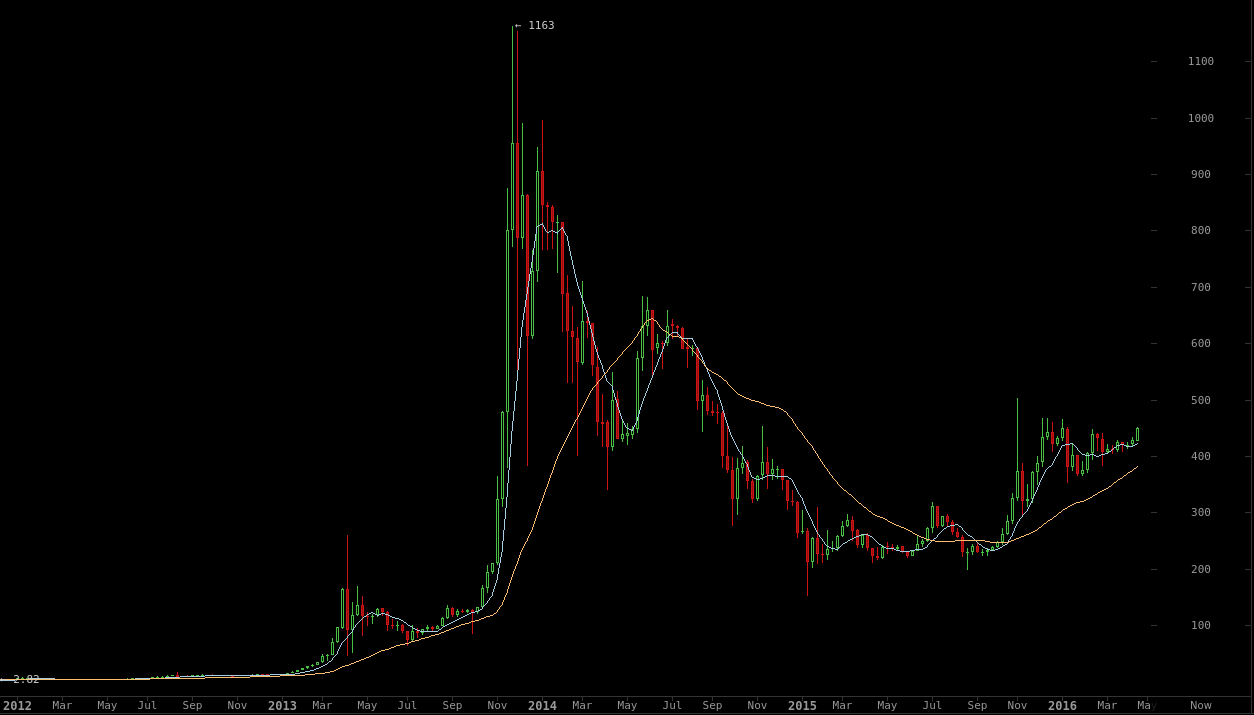
\includegraphics[scale=0.24]{btchodnota.png}
    \caption{Vývoj hodnoty BTC za posledné 4 roky v amerických dolároch}
    \end{figure}
\end{frame}


\begin{frame}[standout]
    Ďakujem za pozornosť! 
\end{frame}
\end{document}
